\section{Feature Selection}

\subsection{Selection Techniques}
One drawback of natural language processing is that your feature space explodes very quickly.
By only using unigrams we already have over 80.000 features.
This increases to in the millions when using bigrams and trigrams as well (\eg a n-gram range of (1,3) gives almost 5 million features).
To deal with this problem there we focused on two techniques that reduces the feature space (1) dimensionality reduction and (2) feature selection through statistical significance.

\mysubsubsection{Latent Semantic Analysis}
A popular approach in the context of natural language processing is Latent Semantic Analysis (LSA). LSA is a form of dimensionality reduction using SVD. It allows us to choose the number of components, which will be the new number of features. LSA tries to limit the loss of information by allowing you to reconstruct the original data as close as possible.


\mysubsubsection{K-Best Features}
Another approach is to compare the features against each other and see which features are statistically insignificant or less important. Finally, all the features are ranked based on their significance and the top K features are then selected to be used in the model. \textit{K} is a parameter that is chosen by the user. We decided to set "K" as 10,000. As seen in Figure~\ref{fig:ngram}, the plot for unigram (blue line) levels out at approx. K=10,000 for the F1-score, Precision as well as Recall.

\subsection{Comparison}
We chose to go with K-Best (with the Chi-square test) feature selection due to it being considerably faster to compute than LSA for larger numbers. Also as we can see that the performance for a dimension of 10 and 100, K-Best does considerably better than LSA, see Figure~\ref{fig:selection-features}. However, we also note that K-Best performs worse when K increases. This seems strange, because more features are allowed to contribute to the model and in previous scenarios, see Figure~\ref{fig:ngram}, we saw an increase in performance when k was increased further. 

Overall, K-Best seems to perform better when looking at the f1-score and when taking training time into account.


\begin{figure*}[ht!]
    \centering
    \subfloat[F1-score for different n-gram ranges\label{fig:ngram-f1}]{%
        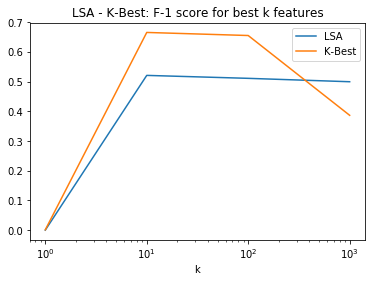
\includegraphics[width=0.3\linewidth]{figures/selection/f1-score-lsa-k.png}}
    \hfill
    \subfloat[Precision-score for different n-gram ranges\label{fig:ngram-precision}]{%
        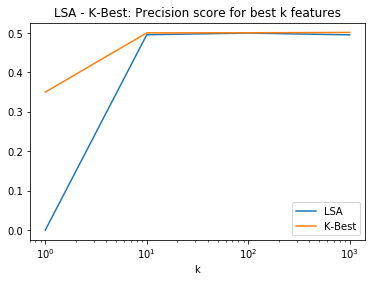
\includegraphics[width=0.3\linewidth]{figures/selection/p-score-lsa-k.png}}
        \hfill
    \subfloat[Recall-score for different n-gram ranges\label{fig:ngram-recall}]{%
        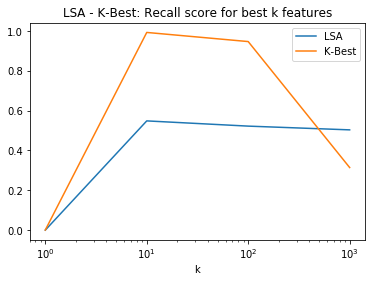
\includegraphics[width=0.3\linewidth]{figures/selection/r-score-lsa-k.png}}
  \caption{Scores for different N-gram ranges.}
  \label{fig:selection-features} 
\end{figure*}